\documentclass[a4paper]{llncs}
\usepackage{graphicx}
\usepackage{longtable}
\usepackage[latin1]{inputenc}
\usepackage{subfigure}
\usepackage{a4wide}
\usepackage{listings}
\usepackage[hyphens]{url}
\urldef{\mails}\path|{ei05011,ei05028}@fe.up.pt|
\bibliographystyle{splncs}
\begin{document}
\title{Progress Report on the ``Adult Database'' Analysis}
\author{Fl�vio Cruz \and Jo�o Azevedo}
\institute{Faculdade de Engenharia da Universidade do Porto\\
    Rua Dr. Roberto Frias, s/n 4200-465 Porto PORTUGAL\\
    \mails}
\maketitle

\begin{abstract}
Highly frequent in experimental tests related to data mining, the Adult Database
has some interesting properties which make it quite useful to test the 
efficiency of classification algorithms. This report aims to describe the Adult
Database from a statistical perspective and taking into account its support for
data mining tasks.
\end{abstract}

\section{Introduction}

Classification in data mining is the activity of identifying a given object as 
belonging to a pre-defined class \cite{1}. The ultimate goal is to learn a concept. This
learning process is based on past observations, where the dataset performs a
main role. This report gives a first overview on the ``Adult Database'' dataset,
describing its format and identifying the problem it poses. Some data analysis
is then done, in order to obtain some characteristics on the global set of
values. Finally, the future work plan is presented and some conclusions on the
subject are taken.

\section{Data Format}

The ``Adult Database'' consists of 48842 entries of individual information of 
people gathered in a 1994 census on the United States of America. From the
global collection of data, a representative sample was collected from people
with ages between 16 and 100 and a final weight above 1.

The data set is divided in two groups: the train set with 32561 records and the test set with 16281 entries.

Each entry is composed by a set of 14 attributes and two classes, identifying
persons who gain more or less than 50K dollars per year. The attributes and types are:

\begin{itemize}
  \item{\textbf{Age}: continuous.}
  \item{\textbf{Workclass}: categorical: [[Private], [Self-emp-not-inc], 
        [Self-emp-inc], [Federal-gov], [Local-gov], [State-gov], [Without-pay], 
        [Never-worked]]}
  \item{\textbf{FNLWGT}: continuous. Represents the final weight. People with 
        the same demographical characteristics should have the same weight.}
  \item{\textbf{Education}: ordinal: [1. [Preschool], 2. [1st-4th], 3. 
        [5th-6th], 4. [7th-8th], 5. [9th < 10th], 6. [11th < 12th], 7. 
        [HS-grad], 8. [Prof-school], 9. [Assoc-acdm], 10. [Assoc-voc], 11.
        [Some-college], 12. [Bachelors], 13. [Masters], 14. [Doctorate]]}
  \item{\textbf{Education-num}: continuous. Is a continuous representation of 
        the \textbf{Education} attribute.}
  \item{\textbf{Marital-status}: categorical: [[Married-civ-spouse], [Divorced],
        [Never-married], [Separated], [Widowed], [Married-spouse-absent],
        [Married-AF-spouse]]}
  \item{\textbf{Occupation}: categorical: [[Tech-support], [Craft-repair],
        [Other-service], [Sales], [Exec-managerial], [Prof-specialty], 
        [Handlers-cleaners], [Machine-op-inspct], [Adm-clerical], 
        [Farming-fishing], [Transport-moving], [Priv-house-serv], 
        [Protective-serv], [Armed-Forces]]}
  \item{\textbf{Relationship}: categorical: [[Wife], [Own-child], [Husband], 
        [Not-in-family], [Other-relative], [Unmarried]]}
  \item{\textbf{Race}: categorial: [[White], [Asian-Pac-Islander], 
        [Amer-Indian-Eskimo], [Other], [Black]]}
  \item{\textbf{Sex}: categorical: [[Male], [Female]]}
  \item{\textbf{Capital-gain}: continuous.}
  \item{\textbf{Capital-loss}: continuous.}
  \item{\textbf{Hours-per-week}: continuous.}
  \item{\textbf{Native-country}: categorical.}
\end{itemize}

There are 3620 records with missing values. The attributes that contain missing values are: \textbf{Workclass}, \textbf{Occupation} and \textbf{Native-country}.

This data set is available in the following URL: \url{ftp://ftp.ics.uci.edu/pub/machine-learning-databases/adult}.

\section{Problem Identification}

Deducing from the previous section, this is a classification problem. Given an adult
with the mentioned attributes we want to classify him into one of the following groups:
one gains more than 50000 dollars per year, the other group does not.

One important objective in classifying things is to understand why the given object
is put under one class and not in another \cite{2}\cite{3}, that is, we want to understand what social characteristics
allows one person to gain more than someone else, if the sex is important, the education level,
the race and what factors are less important.

Given a specific set of persons from a certain society and from a certain time we could then
learn what contributes to a person's social standing and, as we all know, income is an important
metric in that department. We could, for example, learn if the race affects the persons success and if
that society discriminates against certain races.

Understanding what affects the income can give a lot of information concerning society's behaviors.

\section{Data Analysis}

The table \ref{tab:summary} summarizes the distribution of values on the studied
dataset. From a first observation, one can see that the amount of missing values
is low. On the other side, in some of the attributes, some classes have a
much higher frequency than others, such as the 'united-states' native country, 
the 'private' workclass and the 'white' race. On the hours of work per week
attribute, there is a great amount of outliers, with some unrealistic
values, namely with amounts close to the 100 hours or less than 10 in 
individuals with a defined occupation, as can be seen on figure 
\ref{fig:box_hours}. Variables such has the capital gain and capital loss have
few values above 0, being quite specific to certain classes of individuals. The
sex is also unbalanced in the sample data, as the amount of men is more than
twice the amount of women.

It is also important to verify some correlations between variables. To that
matter, we've tested some apparent situations, such as the influence of the age,
hours of work per week and educational level on the amount gained by an
individual. The figures \ref{fig:age_plus50}, \ref{fig:education_plus50} and
\ref{fig:hpw_plus50} show that there is a tendency for older people, people with
a higher educational level and people who work a great amount of hours per week
to gain a larger amount of money.

\subsection{Association Rules}

Using association rules one can find frequent patterns and associations from a
set of transactions. These rules can easily be used to make data analysis and
to understand casual structures.

To build a set of association rules we used the apriori algorithm that is featured
in the R arules package. Before running the algorithm we made some data preprocessing
for continuous attributes that are needed to build better and more general rules.

The following attributes were transformed:

\begin{itemize}
  \item {\textbf{Age}: turned into categories. 15-25 (young), 25-45 (middle\_aged), 45-65 (senior), $>$ 65 (old).}
  \item {\textbf{Hours-per-week}: turned into categories. 0-25 (part\_time), 25-40 (full\_time), 40-60 (overtime), $>$60 (workaholic).}
  \item {\textbf{Capital-gain}: turned into categories. $<=$ 0 (none), $<$ median value (low), $>$ median value (high).}
  \item {\textbf{Capital-loss}: turned into categories. $<=$ 0 (none), $<$ median value (low), $>$ median value (high).}
\end{itemize}

Next, we plotted the relative frequency of items in the transaction database
with support greater than 10\%. The results are shown in figure \ref{fig:arules_item_frequency}.
We can learn various things from that plot: the majority of people are from the united states,
the white race is predominant, males outnumber females and that more people work in full time.

Finally we run the apriori algorithm using the test data set to generate rules
with support greater than 2\% and at least 60\% of confidence. The algorithm built
50487 rules.

We then built two sets of rules from the original set: one with the consequent component
with plus\_50=0 (the person gains less than 50K a year) and the other with plus\_50=1
(the person gains more than 50K a year).

Each rule set was sorted by the confidence level, from more confident to less confident.

The first 5 rules from the plus\_50=0 set are shown in listing \ref{arules_small_income} and
are related to small incomes. We can easily make some observations
about those rules: young people with a part-time are probably low income and having a child
without being married is also not a very good signal.

The second set, contrary to the ones above, shows us the top 5 rules for having large incomes.
These rules are shown in listing \ref{arules_large_income}. A conclusion can readily be made:
being a white husband with a high capital gain probably means we have a large income.

\subsection{Clusters}

Another method to analyze the dataset is based on the generation of clusters. 
Clusters are sets of data in which objects in the same cluster are similar, and
objects in different clusters are dissimilar. The first attempt at clustering
used only three variables: age, education\_num and hours\_per\_week, the same
variables we saw that had a greater impact on the amount gained by the
individual. The data was normalized using the Z-Transformation method and the 
K-Means method was used to obtain the final clusters, with a k of 6, using RapidMiner \cite{4}. Figures 
\ref{fig:cluster_1_age_education}, \ref{fig:cluster_1_education_hpw} and \ref{fig:cluster_1_age_hpw} show
scatter plots of the variables, colored by clusters. One thing one is able to
note is that people with younger age belong to cluster \#2. In terms of
education, people with higher education belong to cluster \#0, while people with
lower education belong to cluster \#1. In terms of hours of work per week, 
distribution is rather similar, but cluster \#2 and \#3 have a greater amount of
lower and higher values, respectively. Figure \ref{fig:cluster_1_cluster_plus50}
shows how clusters relate to the class values. Although the distribution is 
balanced, clusters \#1 and \#2 have a greater amount of people gaining below 
50000 dollars. Notice, as stated before, that this were the clusters having 
people with lower education and younger age, respectively.

Clustering with the remaining attributes leads to results more difficult to
analyze. The same process was applied, using the Z-Transformation method for
normalization and the K-Means algorithm with a k of 6, but this time with all
the attributes. The distribution of values is more balanced, although a very
high value of capital gain, very unusual on the data set, leads to the creation
of a very well identified cluster, as can be seen on table \ref{tab:centroids}.
Particular values of race, workclass and native country also identify clusters
\#2, \#3 and \#2, respectively. Notice that this attributes were the ones
refered to before as having a given value more frequent than others, thus
leading to this particular composition of clusters.

\section{Work plan}

Given the problem at hand, we want to generate a classification mechanism
that can tell if a specific person has a small or large income.

For this we will use various kinds of classification algorithms, from classical
decision trees to rule induction.

We will try to compare the error rate among the various algorithms. We'll be using
the train set to "train" the algorithm and then the test set to assess which algorithm
is best suited to make income predictions.

We'll also use some data-processing techniques to eliminate unknown values. It will
also be useful to categorize continuous values for more generalized rules as we have
done when generating association rules.

The algorithms we will be using are: ID3 \cite{1}, C4.5 \cite{5}, CN2 \cite{1} and AQ \cite{1}. Depending on our progress
we will experiment with neural networks and genetic algorithms, which are other
mechanisms for building classifiers.

\section{Conclusions}

Taking into account the previous analysis of the data, we're now capable of
applying a structured data mining process in order to address the classification
problem posed by the dataset. The final report hopes to compare the performance
and efficiency of different classification algorithms applied to this dataset.
A tentative title for the paper to be delivered as the final report is 
``A comparison of classification algorithms applied to the Adult Database''.

\begin{thebibliography}{1}
\bibitem{1}
Mitchel, T.; Machine Learning; McGraw-Hill, 1997
\bibitem{2}
Han, J., Kamber, M., Pei, J.; Data Mining: Concepts and Techniques, Second Edition; Morgan Kaufmann, 2005
\bibitem{3}
H. Witten, I., Frank, E.; Data Mining: Practical Machine Learning Tools and Techniques, Second Edition; Morgan Kaufmann, 2005
\bibitem{4}
RapidMiner; \url{http://www.rapidminer.com/}, November 2009
\bibitem{5}
Ross Quinlan, J.; C4.5: Programs for Machine Learning; Morgan Kaufmann, 1992
\end{thebibliography}

\clearpage

\appendix

\section{Tables}

\begin{table}
\centering
\subtable[Age]{
       \begin{tabular}{| l | l |}
       \hline
       Min. & 17 \\
       \hline
       1st Qu. & 28 \\
       \hline
       Median & 37 \\
       \hline
       Mean & 38.58 \\
       \hline
       3rd Qu. & 48 \\
       \hline
       Max & 90 \\
       \hline
       \end{tabular}
}
\qquad\qquad
\subtable[Workclass]{        
       \begin{tabular}{| l | l |}
       \hline
       private & 22696 \\
       \hline
       self\_emp\_not\_inc & 2541 \\
       \hline
       local\_gov & 2093 \\
       \hline
       state\_gov & 1298 \\
       \hline
       self\_emp\_inc & 1116 \\
       \hline
       (Other) & 981 \\
       \hline
       NA's & 1836 \\
       \hline
       \end{tabular}
}
\qquad\qquad
\subtable[Education]{        
       \begin{tabular}{| l | l |}
       \hline
       hs\_grad & 10501 \\
       \hline
       some\_college & 7291 \\
       \hline
       bachelors & 5535 \\
       \hline
       masters & 1723 \\
       \hline
       assoc\_voc & 1382 \\
       \hline
       11th & 1175 \\
       \hline
       (Other) & 5134 \\
       \hline
       \end{tabular}
}
\qquad\qquad
\subtable[Marital Status]{        
       \begin{tabular}{| l | l |}
       \hline
       divorced & 4443 \\
       \hline
       married\_af\_spouse & 23 \\
       \hline
       married\_civ\_spouse & 14976 \\
       \hline
       married\_spouse\_absent & 418 \\
       \hline
       never\_married & 10683 \\
       \hline
       separated & 1025 \\
       \hline
       widowed & 993 \\
       \hline
       \end{tabular}
}
\qquad\qquad
\subtable[Occupation]{        
       \begin{tabular}{| l | l |}
       \hline
       prof\_specialty & 4140 \\
       \hline
       craft\_repair & 4099 \\
       \hline
       exec\_managerial & 4066 \\
       \hline
       adm\_clerical & 3770 \\
       \hline
       sales & 3650 \\
       \hline
       (Other) & 10993 \\
       \hline
       NA's & 1843 \\
       \hline
       \end{tabular}
}
\qquad\qquad
\subtable[Relatonship]{        
       \begin{tabular}{| l | l |}
       \hline
       husband & 13193 \\
       \hline
       not\_in\_family & 8305 \\
       \hline
       other\_relative & 981 \\
       \hline
       own\_child & 5068 \\
       \hline
       unmarried & 3446 \\
       \hline
       wife & 1568 \\
       \hline
       \end{tabular}
}
\qquad\qquad
\subtable[Race]{        
       \begin{tabular}{| l | l |}
       \hline
       amer\_indian\_eskimo & 311 \\
       \hline
       asian\_pac\_islander & 1039 \\
       \hline
       black & 3124 \\
       \hline
       other & 271 \\
       \hline
       white & 27816 \\
       \hline
       \end{tabular}
}
\qquad\qquad
\subtable[Sex]{        
       \begin{tabular}{| l | l |}
       \hline
       female & 10771 \\
       \hline
       male & 21790 \\
       \hline
       \end{tabular}
}
\qquad\qquad
\subtable[Capital Gain]{        
       \begin{tabular}{| l | l |}
       \hline
       Min. & 0 \\
       \hline
       1st Qu. & 0 \\
       \hline
       Median & 0 \\
       \hline
       Mean & 1078 \\
       \hline
       3rd Qu. & 0 \\
       \hline
       Max. & 99999 \\
       \hline
       \end{tabular}
}
\qquad\qquad
\subtable[Capital Loss]{        
       \begin{tabular}{| l | l |}
       \hline
       Min. & 0 \\
       \hline
       1st Qu. & 0 \\
       \hline
       Median & 0 \\
       \hline
       Mean & 87.3 \\
       \hline
       3rd Qu. & 0 \\
       \hline
       Max. & 4356 \\
       \hline
       \end{tabular}
}
\qquad\qquad
\subtable[Hours Per Week]{        
       \begin{tabular}{| l | l |}
       \hline
       Min. & 1 \\
       \hline
       1st Qu. & 40 \\
       \hline
       Median & 40 \\
       \hline
       Mean & 40.44 \\
       \hline
       3rd Qu. & 45 \\
       \hline
       Max. & 99 \\
       \hline
       \end{tabular}
}
\qquad\qquad
\subtable[Native Country]{        
       \begin{tabular}{| l | l |}
       \hline
       United States & 29170 \\
       \hline
       Mexico & 643 \\
       \hline
       Philippines & 198 \\
       \hline
       Germany & 137 \\
       \hline
       Canada & 121 \\
       \hline
       (Other) & 1709 \\
       \hline
       NA's & 583 \\
       \hline
       \end{tabular}
}
\qquad\qquad
\subtable[Plus 50]{        
       \begin{tabular}{| l | l |}
       \hline
       No & 24720 \\
       \hline
       Yes & 7841 \\
       \hline
       \end{tabular}
}
\caption{Summary of the value distribution in the database}
\label{tab:summary}
\end{table}

\begin{table}
\centering
\begin{tabular}{ | l | l | l | l | l | l | l | }
\hline
\textbf{Attribute} & \textbf{Centroid \#0} & \textbf{Centroid \#1} & \textbf{Centroid \#2} & \textbf{Centroid \#3} & \textbf{Centroid \#4} & \textbf{Centroid \#5} \\
\hline
age	& -0.874 & 0.692 & -0.166 & 0.246 & 0.570 & 0.190 \\
\hline
workclass & -0.272 & -0.063 & -0.036 & 2.208 & 0.455 & -0.364 \\
\hline
education\_num & -0.101 & -0.172 & -0.177 & 0.0309 & 1.103 & 0.102 \\
\hline
marital\_status & -0.679 & 1.693 & -0.083 & -0.150 & -0.007 & -0.108 \\
\hline
occupation & -0.305 & -0.303 & 0.091 & 0.952 & -0.434 & 0.010 \\
\hline
relationship & 0.703 & 0.526 & 0.189 & -0.053 & -0.351 & -0.507 \\
\hline
race & -0.086 & -0.020 & 2.630 & -0.147 & -0.002 & -0.230 \\
\hline
sex & 0.662 & 1.199 & 0.019 & -0.161 & -0.409 & -0.635 \\
\hline
capital\_gain & -0.116 & -0.091 & -0.086 & -0.029 & 13.394 & -0.040 \\
\hline
capital\_loss & -0.115 & -0.079 & -0.021 & 0.025 & -0.217 & 0.079 \\
\hline
hours\_per\_week & -0.523 & -0.231 & -0.031 &-0.071 & 0.758 & 0.339 \\
\hline
native\_country & -0.186 & -0.154 & 2.951 & -0.181 & -0.075 & -0.171 \\
\hline
\end{tabular}
\caption{Centroid table for the results of the application of the K-Means algorithm with a k of 6}
\label{tab:centroids}
\end{table}

\clearpage

\section{Figures}

\begin{figure}
\centering
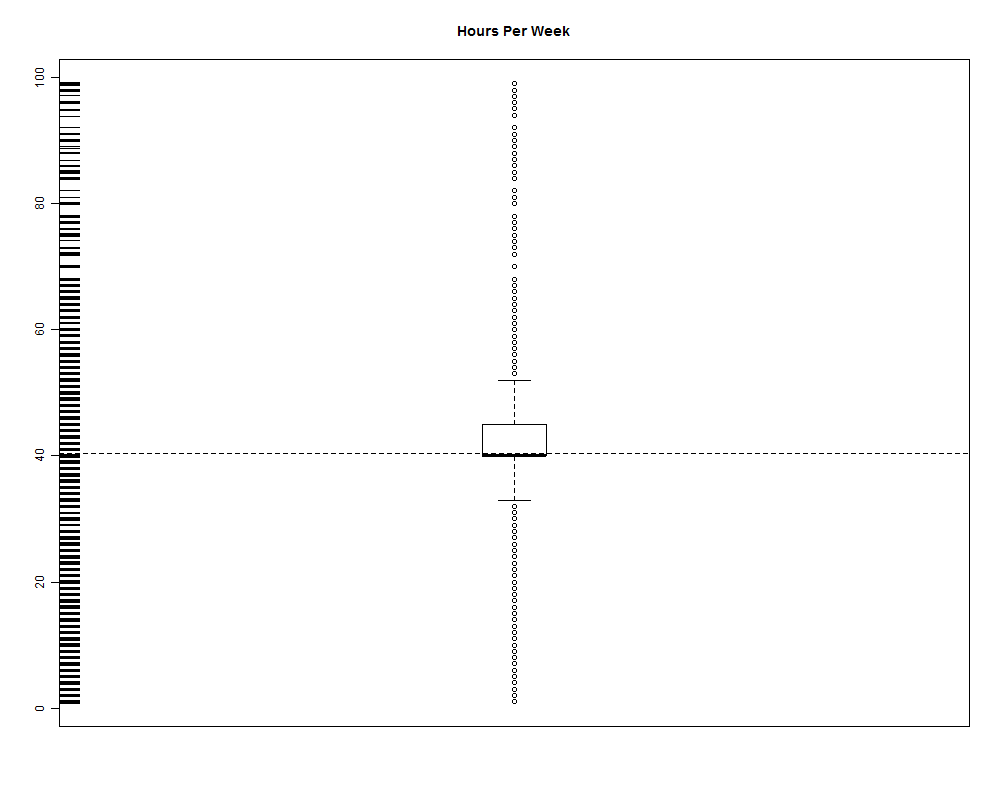
\includegraphics[width=10cm]{boxplot_hours_per_week.png}
\caption{Boxplot of the hours per week variable}
\label{fig:box_hours}
\end{figure}

\begin{figure}
\centering
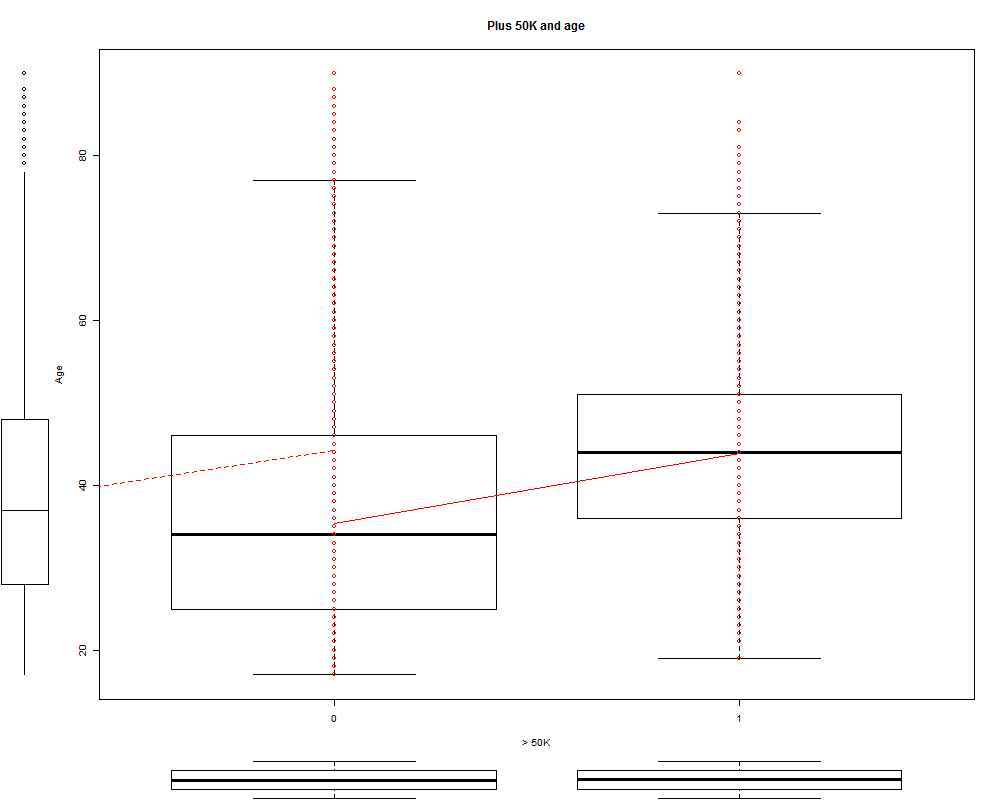
\includegraphics[width=10cm]{plot_plus_50_age.png}
\caption{Boxplot of the individuals' age, for each class of gain}
\label{fig:age_plus50}
\end{figure}

\begin{figure}
\centering
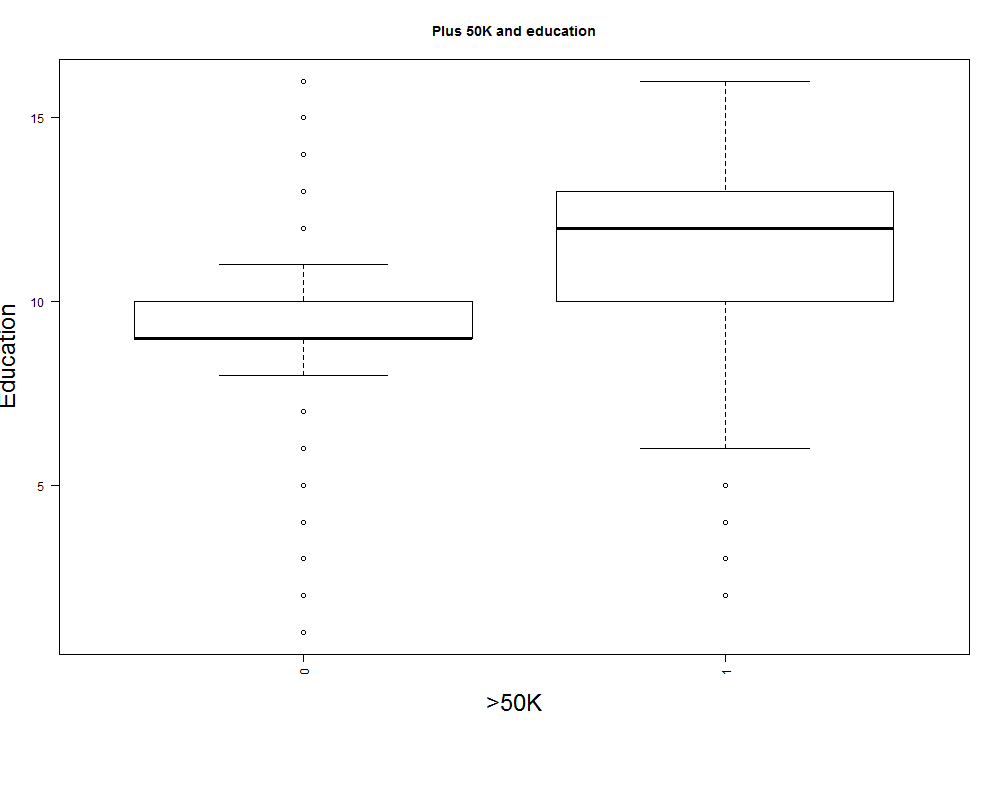
\includegraphics[width=10cm]{plot_plus_50_education_num.png}
\caption{Boxplot of the individuals' education level, for each class of gain}
\label{fig:education_plus50}
\end{figure}

\begin{figure}
\centering
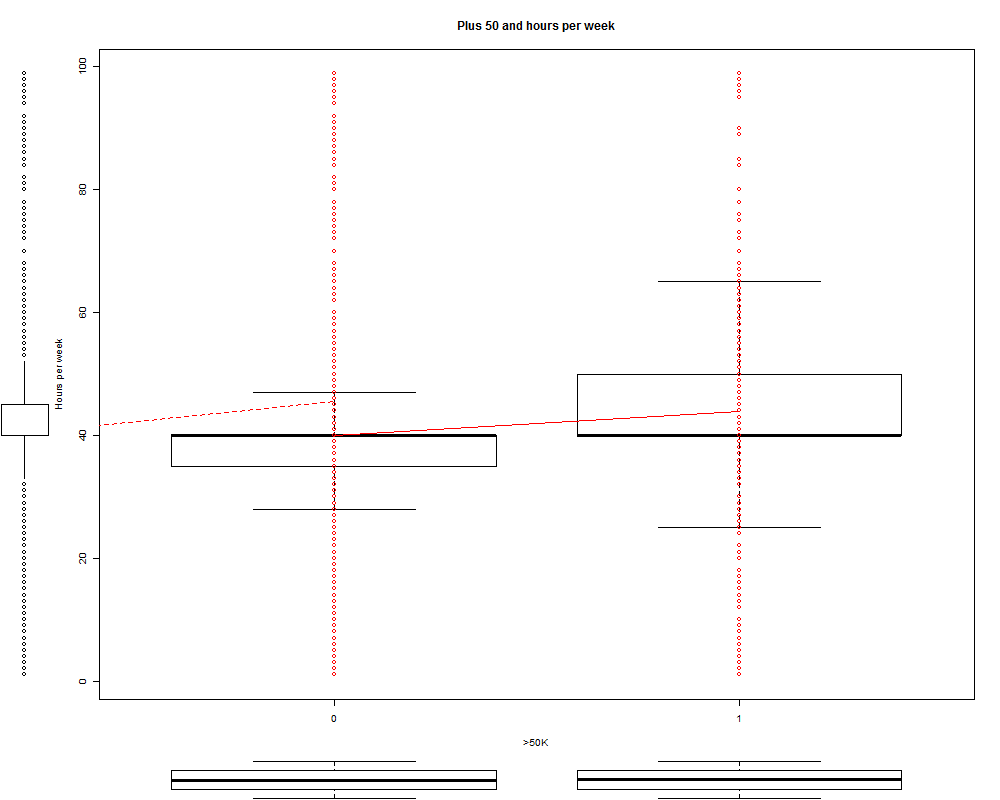
\includegraphics[width=10cm]{plot_plus_50_hpw.png}
\caption{Boxplot of the individuals' hours of work per week, for each class of 
gain}
\label{fig:hpw_plus50}
\end{figure}

\begin{figure}
\centering
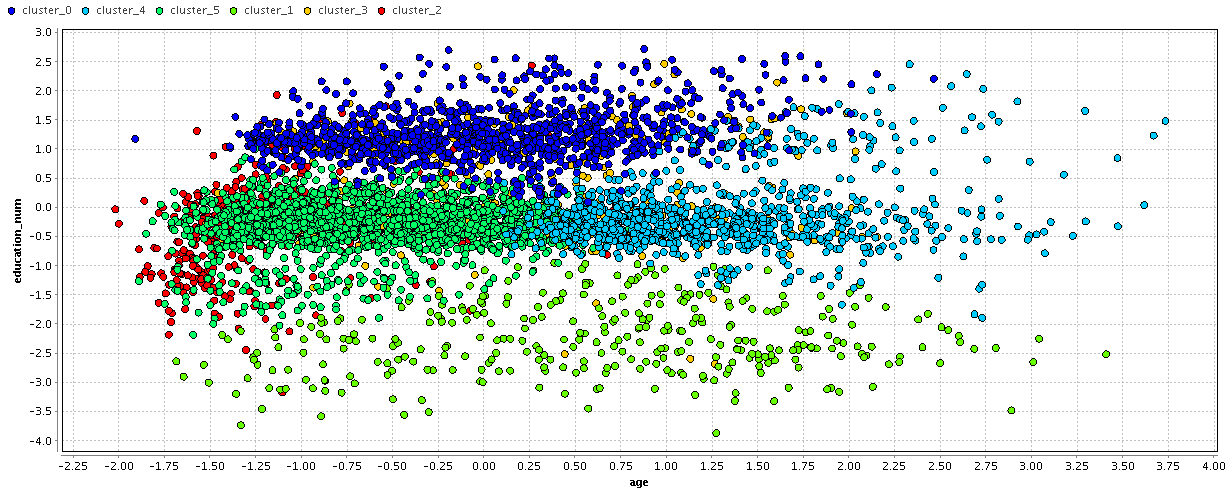
\includegraphics[width=10cm]{cluster_1_age_education.png}
\caption{Scatter plot of age and education}
\label{fig:cluster_1_age_education}
\end{figure}

\begin{figure}
\centering
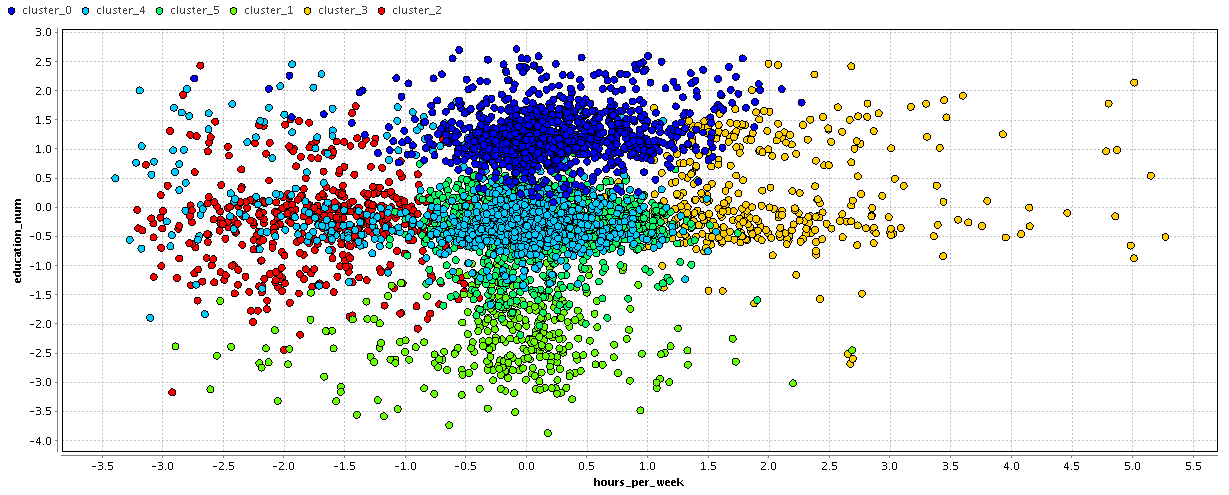
\includegraphics[width=10cm]{cluster_1_education_hpw.png}
\caption{Scatter plot of education and hours of work per week}
\label{fig:cluster_1_education_hpw}
\end{figure}

\begin{figure}
\centering
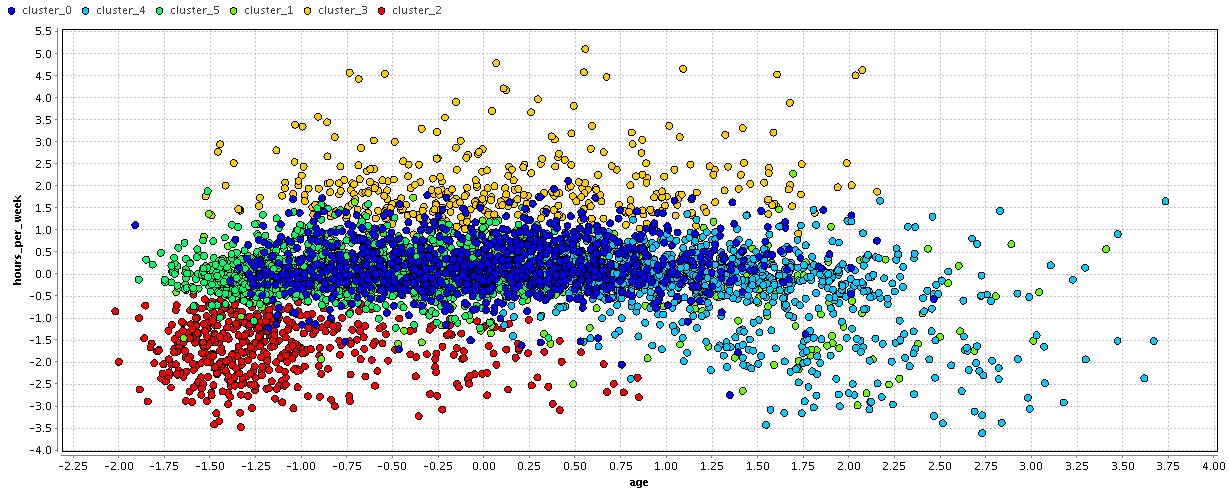
\includegraphics[width=10cm]{cluster_1_age_hpw.png}
\caption{Scatter plot of age and hours of work per week}
\label{fig:cluster_1_age_hpw}
\end{figure}

\begin{figure}
\centering
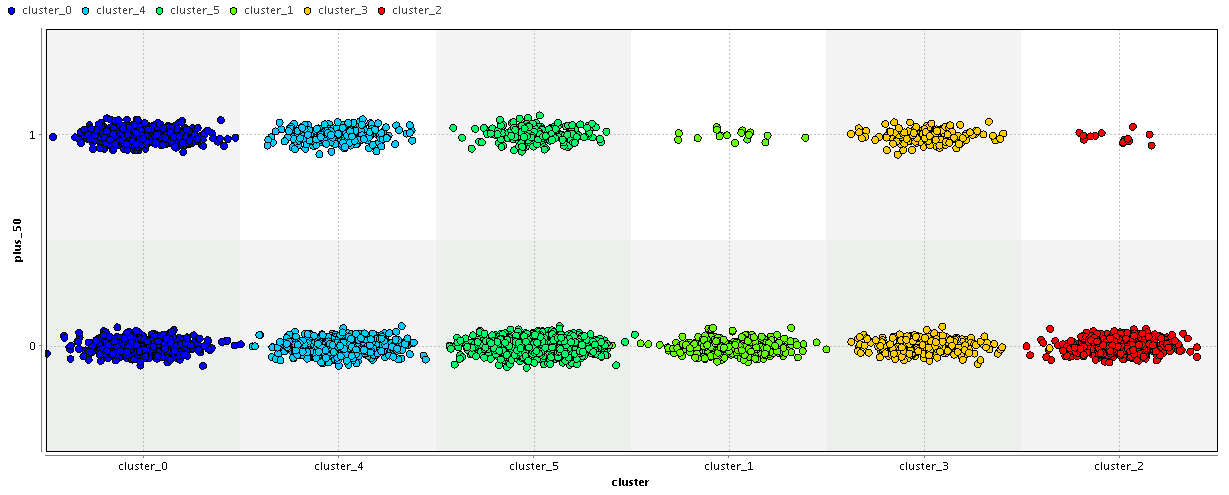
\includegraphics[width=10cm]{cluster_1_cluster_plus50.png}
\caption{Scatter plot of cluster and class values of amount gained}
\label{fig:cluster_1_cluster_plus50}
\end{figure}

\begin{figure}
\centering
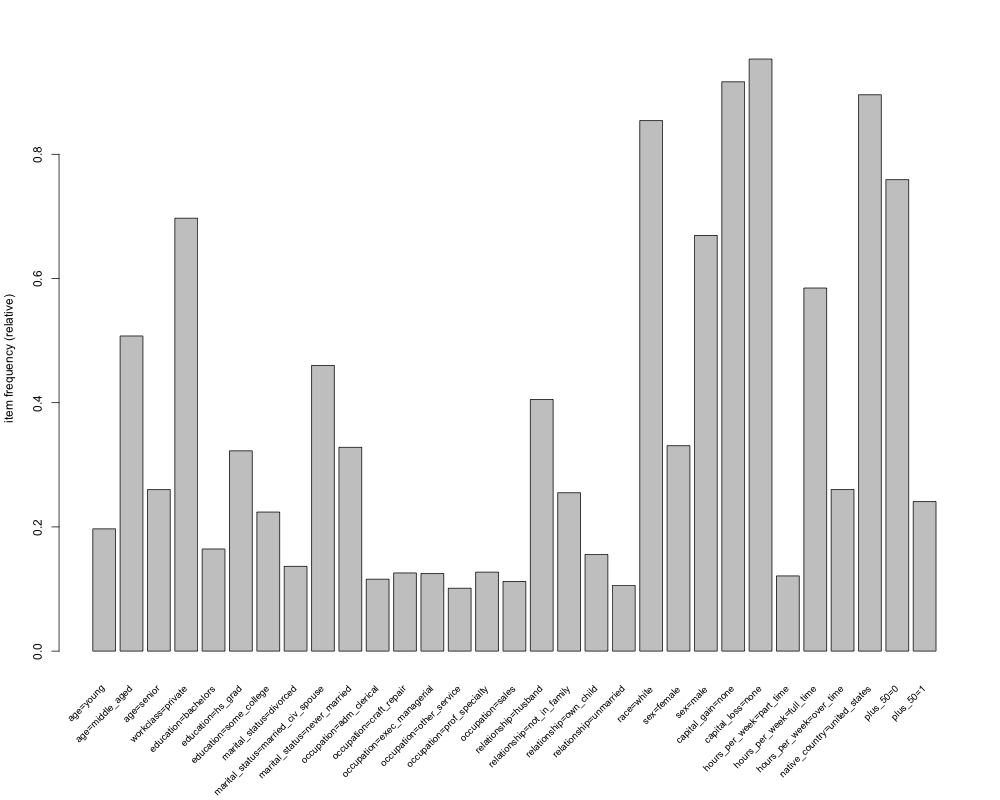
\includegraphics[width=20cm,angle=90]{item_frequency.png}
\caption{Item frequencies of items with at least 10\% support.}
\label{fig:arules_item_frequency}
\end{figure}

\clearpage
\section{Listings}

\begin{lstlisting}[language=r,frame=single,breaklines=true,basicstyle=\footnotesize\ttfamily,caption={Association rules for small income.},label=arules_small_income]
  lhs                               rhs            support confidence     lift
1 {age=young,                                                                 
   hours_per_week=part_time}     => {plus_50=0} 0.05730782          1 1.317193
2 {age=young,                                                                 
   occupation=unknown,                                                        
   capital_gain=none}            => {plus_50=0} 0.02002396          1 1.317193
3 {age=young,                                                                 
   relationship=own_child,                                                    
   hours_per_week=part_time}     => {plus_50=0} 0.04404042          1 1.317193
4 {education=some_college,                                                    
   relationship=own_child,                                                    
   hours_per_week=part_time}     => {plus_50=0} 0.02069961          1 1.317193
5 {marital_status=never_married,                                              
   relationship=own_child,                                                    
   hours_per_week=part_time}     => {plus_50=0} 0.04689659          1 1.317193
\end{lstlisting}

\begin{lstlisting}[language=r,frame=single,breaklines=true,basicstyle=\footnotesize\ttfamily,caption={Association rules for large income.},label=arules_large_income]
  lhs                                    rhs            support confidence     lift
1 {relationship=husband,                                                           
   race=white,                                                                     
   capital_gain=high}                 => {plus_50=1} 0.02063819  0.9926145 4.121990
2 {marital_status=married_civ_spouse,                                              
   relationship=husband,                                                           
   race=white,                                                                     
   capital_gain=high}                 => {plus_50=1} 0.02063819  0.9926145 4.121990
3 {relationship=husband,                                                           
   race=white,                                                                     
   sex=male,                                                                       
   capital_gain=high}                 => {plus_50=1} 0.02063819  0.9926145 4.121990
4 {relationship=husband,                                                           
   race=white,                                                                     
   capital_gain=high,                                                              
   capital_loss=none}                 => {plus_50=1} 0.02063819  0.9926145 4.121990
5 {relationship=husband,                                                           
   capital_gain=high}                 => {plus_50=1} 0.02251159  0.9918809 4.118943
\end{lstlisting}

\end{document}
